%%%
%
% $Autor: Wings $
% $Datum: 2021-05-14 $
% $Pfad: GitLab/MLEdgeComputer $
% $Dateiname: 
% $Version: 4620 $
%
% !TeX spellcheck = en_EN-EnglishUnitedKingdom
% !TeX program = pdflatex
% !BIB program = biber/bibtex
% !TeX encoding = utf8
%
%%%



\chapter{Project Magic Wand}

\section{Sources}




\begin{itemize}
    \item Hier findet man auch die librariy TensorFlow Lite: \URL{https://codelabs.developers.google.com/magicwand}
    \item \URL{https://github.com/tensorflow/tflite-micro-arduino-examples/tree/main}
    \item Auch interessant, aber nicht klar wozu:\URL{https://github.com/tensorflow/tflite-micro/}
    \item check this link: \URL{https://www.tensorflow.org/lite/microcontrollers}
\end{itemize}




\section{Introduction} 


The objective of this chapter is to create a project ``Magic Wand'' and implement the same into a board Arduino Nano BLE33 Sense. Gestures namely ``Wing'', ``Ring'' and ``Slope'' will be recognized by the board when the wand is waved. The direction of motion for the recognition of the gestures are shown in the figure \ref{gestures}.

    
    \begin{center} 
        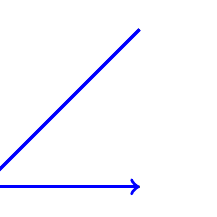
\begin{tikzpicture}
            % define point
            \hspace{-0.6cm}
            \coordinate (A)  at (2, 2);
            \coordinate (O)  at (0, 0);
            \coordinate (B)  at (2, 0);
            % angle  
            \draw[thick] (A) -- (O) -- (B);
            %\draw pic[draw=black,angle radius=20,angle eccentricity=1.4]
            %{angle = B--O--A};
            %\pic [draw,"$\alpha_1$",angle radius=20,->,angle eccentricity=1.4]
            %  {angle = B--O--A};
            \draw [->, very thick,blue] (2,2) -- (0,0)  node [midway, above] {\scriptsize };
            \draw [->, very thick,blue] (0,0) -- (2,0)  node [midway, above] {\scriptsize };
        \end{tikzpicture}
        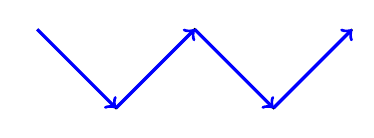
\begin{tikzpicture}
            \hspace{0.1cm}
            % define point
            \coordinate (A)  at (1, 1);
            \coordinate (O)  at (2, 0);
            \coordinate (B)  at (3, 1);
            \coordinate (C)  at  (4,0);
            \coordinate (D) at  (5,1);
            % angle  
            \draw[thick] (A) -- (O) -- (B) -- (C)-- (D);
            %	\draw pic[draw=black,eccentricity=2.9]
            %\pic [draw,"$\alpha_1$",angle radius=20,->,angle eccentricity=1.4]
            %  {angle = B--O--A};
            \draw [->, very thick,blue] (1,1) -- (2,0)  node [midway, above] {\scriptsize };
            \draw [->, very thick,blue] (2,0) -- (3,1)  node [midway, above] {\scriptsize };
            \draw [->, very thick,blue] (3,1) -- (4,0)  node [midway, above] {\scriptsize };
            \draw [->, very thick,blue] (4,0) -- (5,1)  node [midway, above] {\scriptsize };
        \end{tikzpicture}
        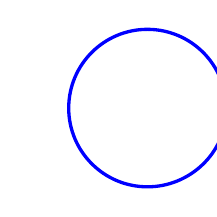
\begin{tikzpicture}
            \hspace{0.5cm}
            \draw[->,very thick,blue] (0,0) arc[radius=1cm,start angle=0,delta angle=359];
        \end{tikzpicture}
        \captionof{figure}{Gestures used namely ``Slope'', ``Wing'' and ``Ring''} \label{gestures} 
    \end{center} 

When the wand is moved in the direction as shown in the figure, the gesture interpreted by the board is transformed into a visual output. 
The board Arduino Nano 33 BLE Sense is be programmed such that the \ac{led}  blinks according to the commands given in relation to the gestures waved by the hand. Here, the Arduino is programmed to indicate a green light when a ``Wing'' is waved, red for ``Slope'' and,  blue for ``Ring''. In case any of the gestures are not recognized, there will also be an output to notify that the gesture is ``Unknown''.


To construct magic wand, attach the board Arduino Nano BLE 33 Sense to the end of a stick, see figure~\ref{MagicWand}. Then feed the accelerometer's output into a deep learning model, which will perform classification to tell whether a known gesture was made. \cite{Warden:2020}

\begin{center}
    
\includegraphics[width=\textwidth]{MagicWand/MagicWandPhoto}
    
    \captionof{figure}{Magic Wand}\label{MagicWand}
\end{center}

\Mynote{Picture of the magic wand}

Gestures collected using the built-in multi-dimensional sensor on the board Arduino Nano 33 BLE Sense are able to understand the complex data and the model can be trained such that it understands the complex data and embeds them in to the  microcontroller. Specifically, it uses TensorFlow Lite \Mynote{cite} to run Convolutional Neural Network model to recognize gestures with an accelerometer.  If the model detects the movements correct, the result is presented in the Arduino IDE's serial monitor.


\Mynote{structure?}

\section{Descriptions of the gestures}

\textcolor{red}{\begin{itemize}
    \item Postion of the stick? Horizontal? Vertical?
    \item Speed?
    \item Time?
    \item Direction?
    \item \ldots
\end{itemize}
}


The Magic Wand project check about 4 gestures for each gesture we have specific color: 

\begin{itemize}
    
    \item Gesture Wing: color red
    \item Gesture Ring: color green 
    \item Gesture Slope: color blue
    \item Gesture Unknown : color red/green/blue with 0.5 seconde ON/OFF on each color
\end{itemize}


\subsection{Gesture Wing}

The first set of data that we are trying to capture the movement is for the gesture Wing. The steps involved  is mentioned below.

\begin{center}
    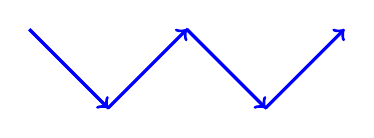
\begin{tikzpicture}
        % define point
        \coordinate (A)  at (1, 1);
        \coordinate (O)  at (2, 0);
        \coordinate (B)  at (3, 1);
        \coordinate (C)  at  (4,0);
        \coordinate (D) at  (5,1);
        % angle  
        \draw[thick,blue] (A) -- (O) -- (B) -- (C)-- (D);
        \draw [->, very thick,blue] (1,1) -- (2,0)  node [midway, above] {\scriptsize };
        \draw [->, very thick,blue] (2,0) -- (3,1)  node [midway, above] {\scriptsize };
        \draw [->, very thick,blue] (3,1) -- (4,0)  node [midway, above] {\scriptsize };
        \draw [->, very thick,blue] (4,0) -- (5,1)  node [midway, above] {\scriptsize };
    \end{tikzpicture}
    \captionof{figure}{Gesture Wing}
\end{center}


The letter \textbf{W} is composed by 4 little movement : 

\begin{itemize}
    \item The device is first moved down and to the right.
    \item Then the device is moved up and to the right.
    \item The device is then moved down and to the right.
    \item  The device is then moved up and to the right again. 
\end{itemize}


\subsection{Gesture Ring}

The gesture Ring is composed by circular motion.  

\begin{center}
    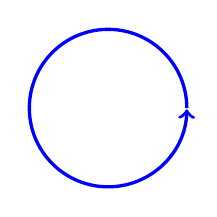
\begin{tikzpicture}
        \draw[->,very thick,blue] (0,0) arc[radius=1cm,start angle=0,delta angle=359];
    \end{tikzpicture}
    
    \captionof{figure}{Gesture Ring}	
\end{center}

The process involved in capturing gesture Ring are as follows.

\begin{itemize}
    \item Trace a clockwise circle using the wand.
    \item Aim again to take around a second to perform gesture.	
    \item The gesture Ring is a rotation of wirst and not shoulder.
\end{itemize}


\subsection{Gesture Slope}

\begin{center}	
    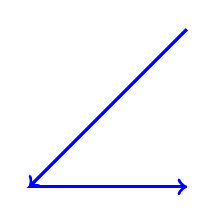
\begin{tikzpicture}	
        \coordinate (A)  at (2, 2);
        \coordinate (O)  at (0, 0);
        \coordinate (B)  at (2, 0);
        
        \draw[thick,blue] (A) -- (O) -- (B);
        \draw [->, very thick,blue] (2,2) -- (0,0)  node [midway, above] {\scriptsize };
        \draw [->, very thick,blue] (0,0) -- (2,0)  node [midway, above] {\scriptsize };
    \end{tikzpicture}
    
    \captionof{figure}{Gesture Slope}
    
\end{center}
The steps involved in waving the gesture Slope  is mentioned below.
\begin{itemize}
    
    \item The device is first moved down and to the left.
    \item Then the device is moved to the right.
    \item Finally you should get a corner of the triangle as shown in the figure.
    
\end{itemize}

The movement recognized is possible after train each part, each movement. If we do Slope on left or on right it's different movement.

Some problem can appart when you try to do the movement, the problem  is the gesture Slope is always detect. 

The movements based on Wrist and shoulder are different, although they can give similar results, so it's essential to focus on training. Depending on the training, one of the two will stand out. 



\section{Database: Collection and Creation}

Since there are no existing databases for the model a new database will be created. The database is a file \FILE{*.txt} which contains raw data from the accelerator  readings recognized by the Arduino Nano 33 BLE Sense. Since the way how the gesture is recorded by a person varies from one to another, gestures of three people are recorded. In order for the database to have a vast amount of data, each person will record a minimum of 50 trials for each gesture. This would improve the efficiency and  effectiveness of the database making it more concrete. 

There is also a possibility to add further data into our model which would improve our model over time.The size of the database thus created will be very small that would be less than 2 MB. \cite{Warden:2020}


For the Magic Wand project, the dataset was meticulously crafted using the sketch Magic Wand Capture \Mynote{filename?} on an Arduino Nano 33 BLE Sense board. The following steps outline the process:

\begin{enumerate}
    
    \item \textbf{Upload the sketch Magic Wand Capture:}
    
    Utilized the sketch Magic Wand Capture, specifically designed for boards Arduino Nano 33 BLE Sense, to record sensor readings during gesture performances.
    
    Uploaded the sketch Magic Wand Capture onto the board Arduino Nano 33 BLE Sense board. This sketch is responsible for collecting and logging accelerometer data during wand movements with the help of tinyml  \href{https://tinyml.seas.harvard.edu/magic_wand/}{website}.\Mynote{cite!}
    
    The website \url{https://tinyml.seas.harvard.edu/magic_wand/} serves as a platform for the project Magic Wand, providing resources and tools for capturing and creating gesture datasets. Users can upload the sketch Magic Wand Capture to a board Arduino Nano 33 BLE Sense, connect it to a laptop via Bluetooth, and record distinct gestures.
    
    \item \textbf{Bluetooth Connectivity:}
    
    Established a connection between the board Arduino Nano 33 BLE Sense and a laptop using the integrated Bluetooth module. This connection facilitated real-time data transfer between the board and the laptop \ref{Fig: Bluetooth Connection}.
    
    \begin{figure}[h!]
        
        \centering
        
\includegraphics[width=100mm]{MagicWand/Bluetoothconnection}
        \caption{Connecting the Arduino Nano BLE 33 Sensor through Bluetooth to create our own Dataset} 
        \label{Fig: Bluetooth Connection}
    \end{figure}
    
    \item \textbf{Gesture Recording:}
    
    Waved the wand in distinct patterns to represent different gestures (W, O, and L).
    The accelerometer on the board captured the corresponding motion data in three dimensions (X, Y, Z) on the screen in real time.
    
    The first set of data that we are trying to capture the movement is for the gesture \textbf{W}. The steps involved  is mentioned below.
    
    \begin{center}
        
        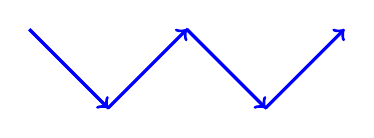
\begin{tikzpicture}
            % define point
            \coordinate (A)  at (1, 1);
            \coordinate (O)  at (2, 0);
            \coordinate (B)  at (3, 1);
            \coordinate (C)  at  (4,0);
            \coordinate (D) at  (5,1);
            % angle  
            \draw[thick,blue] (A) -- (O) -- (B) -- (C)-- (D);
            \draw [->, very thick,blue] (1,1) -- (2,0)  node [midway, above] {\scriptsize };
            \draw [->, very thick,blue] (2,0) -- (3,1)  node [midway, above] {\scriptsize };
            \draw [->, very thick,blue] (3,1) -- (4,0)  node [midway, above] {\scriptsize };
            \draw [->, very thick,blue] (4,0) -- (5,1)  node [midway, above] {\scriptsize };
        \end{tikzpicture}
        
        \captionof{figure}{\textbf{Wing Gesture \cite{Warden:2020}}}
        
    \end{center}
    
    \begin{itemize}
        
        \item The device is first moved down and to the right.
        
        \item Then the device is moved up and to the right.
        
        \item The device is then moved down and to the right.
        
        \item  The device is then moved up and to the right again. 
        
    \end{itemize}
    
    Shows a sample of real data captured during the "wing" gesture, measured in milli-Gs.  
    The process involved in capturing a ring are as follows. \cite{Warden:2020}
    
    \begin{center}
        
        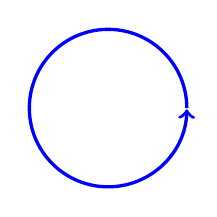
\begin{tikzpicture}
            
            \draw[->,very thick,blue] (0,0) arc[radius=1cm,start angle=0,delta angle=359];
            
        \end{tikzpicture}
        
        \captionof{figure}{\textbf{Ring Gesture \cite{Warden:2020}}}
        
    \end{center}
    
    \begin{itemize}
        
        \item Trace a clockwise circle using the wand.
        
        \item Aim again to take around a second to perform gesture.
        
    \end{itemize}
    
    The steps involved in waving the slope gesture is mentioned below \cite{Warden:2020}:.
    
    \begin{center}
        
        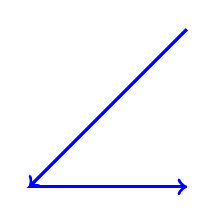
\begin{tikzpicture}
            % define point
            \coordinate (A)  at (2, 2);
            \coordinate (O)  at (0, 0);
            \coordinate (B)  at (2, 0);
            % angle  
            \draw[thick,blue] (A) -- (O) -- (B);
            %\draw pic[draw=black,angle radius=20,angle eccentricity=1.4]
            %{angle = B--O--A};
            %\pic [draw,"$\alpha_1$",angle radius=20,->,angle eccentricity=1.4]
            %  {angle = B--O--A};
            \draw [->, very thick,blue] (2,2) -- (0,0)  node [midway, above] {\scriptsize };
            \draw [->, very thick,blue] (0,0) -- (2,0)  node [midway, above] {\scriptsize };
        \end{tikzpicture}
        
        \captionof{figure}{\textbf{Slope Gesture \cite{Warden:2020}}}
        
    \end{center}
    
    \begin{itemize}
        
        \item The device is first moved down and to the left.
        
        \item Then the device is moved to the right.
        
        \item Finally you should get a corner of the triangle as shown in the figure.
        
    \end{itemize}
    
    The process is repeated until around 250 readings are captured by the wand for Data Preparation and Transformation. 
    
    In order to consider the unknown readings, we have decided that the gesture other than W, O and L are unknown. This would help the wand recognize any unknown gesture and gives the output stating that it is false. \cite{Warden:2020}
    
    All readings that are recorded in a unique JSON file for each gesture. The files \FILE{.json} contains raw accelerometer data that would later be transformed in to machine learning language that should be interpreted by the compiler.
    
    \begin{figure}[h!]
        
        \centering
        
\includegraphics[width=100mm]{MagicWand/Creatingdataset}
        \caption{Creating and collecting the data by moving the sensor to get correct gesture } 
        \label{Fig: Collecting the Data}
        
    \end{figure}
    
    \item \textbf{Labeling Process:}
    
    Reviewed the recorded gestures on the laptop screen and labeled each gesture with the corresponding gesture name (W, O, or L) by clicking on the  symbol ``?'' in the user interface \ref{Fig: Collecting the Data}.
    
    \item \textbf{Error Correction:}
    
    Identified and corrected mistakes by removing any mislabeled or ambiguous instances, ensuring the dataset's quality.
    
    \item \textbf{Download as JSON:}
    
    Downloaded the labeled gestures as a JSON data file using the provided functionality on the project \href{https://tinyml.seas.harvard.edu/magic_wand/}{website}. This file served as the foundation for model training.
    \Mynote{structure?}
\end{enumerate}

\section{Data Preparation}

%%%%%%%%%%%%%%%%%%%%%%%%%%%%%%%

With the data available for the gestures, we can use it to train a model. The data that is available is split in to two namely as training data and test data.
\Mynote{How?}

The major challenge while preparing data can be the presence of outliers or anomalies where there are unexpected values. This can be overcome by feeding our model with more data so that the model is efficient. \cite{Warden:2020}

The different steps involved in preparing data can be as follows according to \cite{Warden:2020}


The step deals with converting the raw data in to machine learning language that can be interpreted by the compiler. \Mynote{How?}
 


Since the amount of data required for creation of a database is very small the database will be prepared by us. The first set of data that we are trying to capture the movement is for the gesture ``W''. The steps involved in capturing a ``W'' is mentioned below. \cite{Warden:2020}

\begin{center}
    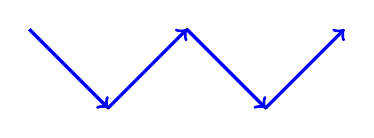
\begin{tikzpicture}
        % define point
        \coordinate (A)  at (1, 1);
        \coordinate (O)  at (2, 0);
        \coordinate (B)  at (3, 1);
        \coordinate (C)  at  (4,0);
        \coordinate (D) at  (5,1);
        % angle  
        \draw[thick] (A) -- (O) -- (B) -- (C)-- (D);
        %	\draw pic[draw=black,eccentricity=2.9]
        %\pic [draw,"$\alpha_1$",angle radius=20,->,angle eccentricity=1.4]
        %  {angle = B--O--A};
        \draw [->, very thick,blue] (1,1) -- (2,0)  node [midway, above] {\scriptsize };
        \draw [->, very thick,blue] (2,0) -- (3,1)  node [midway, above] {\scriptsize };
        \draw [->, very thick,blue] (3,1) -- (4,0)  node [midway, above] {\scriptsize };
        \draw [->, very thick,blue] (4,0) -- (5,1)  node [midway, above] {\scriptsize };
    \end{tikzpicture}
    \captionof{figure}{Wing Gesture}
\end{center}


\begin{itemize}
    
    \item The device is first moved down and to the right.
    \item Then the device is moved up and to the right.
    \item The device is then moved down and to the right.
    \item  The device is then moved up and to the right again. 
    
\end{itemize}

The figure \ref{} shows a sample of real data captured during the gesture ``Wing'', measured in mG.  \Mynote{Image is missing}

\begin{center}
    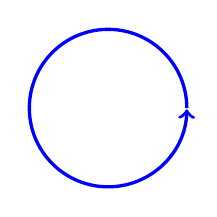
\begin{tikzpicture}
        \draw[->,very thick,blue] (0,0) arc[radius=1cm,start angle=0,delta angle=359];
    \end{tikzpicture}
    \captionof{figure}{\textbf{Ring Gesture \cite{Warden:2020}}}
\end{center}

\begin{itemize}
    \item Trace a clockwise circle using the wand.
    
    \item Aim again to take around a second to perform gesture.
    
\end{itemize}



The steps involved in waving the gesture ``Slope'' is mentioned below \cite{Warden:2020}:

\begin{center}
    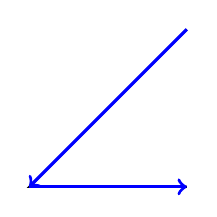
\begin{tikzpicture}
        % define point
        \coordinate (A)  at (2, 2);
        \coordinate (O)  at (0, 0);
        \coordinate (B)  at (2, 0);
        % angle  
        \draw[thick] (A) -- (O) -- (B);
        %\draw pic[draw=black,angle radius=20,angle eccentricity=1.4]
        %{angle = B--O--A};
        %\pic [draw,"$\alpha_1$",angle radius=20,->,angle eccentricity=1.4]
        %  {angle = B--O--A};
        \draw [->, very thick,blue] (2,2) -- (0,0)  node [midway, above] {\scriptsize };
        \draw [->, very thick,blue] (0,0) -- (2,0)  node [midway, above] {\scriptsize };
    \end{tikzpicture}
    \captionof{figure}{\textbf{Slope Gesture \cite{Warden:2020}}}
\end{center}

\begin{itemize}
    \item The device is first moved down and to the left.
    \item Then, the device is moved to the right.
    \item Finally you should get a corner of the triangle as shown in the figure.
\end{itemize}



The process is repeated until around 50 readings are captured by the wand.


\bigskip

In order to consider the unknown readings, we will be carrying out an other set of procedures to feed with unknown data. This would help the wand recognize any unknown gesture and gives the output stating that it is false. \cite{Warden:2020}

\Mynote{Is this necessary?}


\section{Data Characteristics}

\begin{enumerate}
    
    \item \textbf{Size:}
    
    The dataset consists of a total of 250 labeled instances, with over 70 instances for each gesture type (W, O, L).
    
    \item \textbf{Format:}
    
    The dataset is stored in JSON format, a versatile and widely used data interchange format. The JSON structure includes stroke indices, stroke points, and associated X-Y coordinates for each point.
    
    \item \textbf{Structure:}
    
    The JSON structure is organized into strokes, each containing an index and an array of stroke points with X-Y coordinates. This structured format is conducive to representing sequential information.
    
    \begin{lstlisting}
        {
            "gesture_data": [
            {
                "label": "W",
                "sensor_readings": [
                {"acceleration_x": 0.23, "acceleration_y": -0.15, "acceleration_z": 0.98, ...},
                {"acceleration_x": 0.21, "acceleration_y": -0.18, "acceleration_z": 0.95, ...},
                ...
                ]
            },
            {
                "label": "O",
                "sensor_readings": [
                {"acceleration_x": 0.14, "acceleration_y": 0.22, "acceleration_z": 0.93, ...},
                {"acceleration_x": 0.12, "acceleration_y": 0.20, "acceleration_z": 0.91, ...},
                ...
                ]
            },
            {
                "label": "L",
                "sensor_readings": [
                {"acceleration_x": -0.10, "acceleration_y": -0.25, "acceleration_z": 0.88, ...},
                {"acceleration_x": -0.12, "acceleration_y": -0.28, "acceleration_z": 0.85, ...},
                ...
                ]
            },
            ...
            ]
        }
        
    \end{lstlisting}
    
    \item \textbf{Anomalies:}
    
    Emphasized clear and distinct wand movements during gesture performances to reduce anomalies. Applied manual review during the labeling process to identify and rectify any mislabeled or ambiguous instances.
    
    \item  \textbf{Measurement and Screen Size:}
    
    \begin{itemize}
        
        \item Accelerometer Measurements:
        
        The accelerometer on the Arduino Nano 33 BLE Sense board captured motion data in three dimensions (X, Y, Z) during each gesture with the speed of 1 to 2 seconds for a gesture. 
        
        \item Screen Size:
        
        The laptop screen was utilized for real-time visualization that is 25X30 cm dimension and labeling of the recorded gestures. The user interface provided a platform to review, label, and correct the gestures.
        
    \end{itemize}
    
    \item \textbf{Origin:}
    
    The origin of our Magic Wand project dataset lies in the convergence of real-world gestures and cutting-edge technology facilitated by the \href{https://tinyml.seas.harvard.edu/magic_wand/}{website}. Through the collaborative efforts of our team, we employed the Magic Wand Capture sketch, uploading it onto the Arduino Nano 33 BLE Sense board. Leveraging the user-friendly interface provided by the website, we seamlessly recorded, reviewed, and labeled distinct gestures, ensuring a diverse dataset representative of various users and authentic real-world conditions. The Magic Wand prototype, in tandem with the Arduino Nano 33 BLE Sense board, served as the foundation for capturing nuanced variations in gestures. The website's structured approach played a pivotal role in refining our dataset, aligning with the core objectives of our Magic Wand project and enhancing its applicability to practical machine learning applications.
    
\end{enumerate}

The advantage of creating a database with more inputs is that it allows the machine learning model to be more accurate and provide better and more efficient results. The exact process is repeated for the remaining gestures, namely ring, slope, and unknown. With the data available for the above gestures, we can use it to train a model. The available data is split into two: training data and test data.

The major challenge while preparing data can be the presence of outliers or anomalies with unexpected values. This can be overcome by feeding our model with more data so that the model is efficient. Here are some main types of outliers that may be encountered:\cite{Munoz:2019}

\begin{itemize}
    
    \item \textbf{Noise in Accelerometer Readings:}
    
    Environmental noise or interference during data collection can introduce outliers in accelerometer readings. Sudden spikes or drops in sensor values that do not correspond to actual gestures may be considered noise outliers. 
    
    \item  \textbf{Abnormal Gesture Patterns:}
    
    Outliers may occur when users perform gestures outside the expected range or in an unusual manner. These deviations from the standard gesture patterns can impact the model's training and recognition capabilities.
    
    \item \textbf{Sensor Malfunctions:}
    
    Outliers might be caused by sensor malfunctions or inaccuracies in the Arduino Nano 33 BLE Sense device. Sudden jumps, constant offsets, or erratic behavior in sensor readings may indicate hardware issues.
    
    \item \textbf{Inconsistent Data Recording:}
    
    Variability in the way users record gestures, such as differences in speed, amplitude, or duration, can introduce outliers. Harmonizing the dataset by addressing these inconsistencies is essential for training a robust and generalized gesture recognition model.
    
    \item \textbf{User-Specific Outliers:}
    
    Each user may exhibit unique movement patterns or unintentional variations in how gestures are performed. Identifying and addressing user-specific outliers is crucial for creating a model that generalizes well across different individuals within the user group.
    
    \item \textbf{Data Transmission Errors:}
    
    During data transmission from the Arduino Nano to the recording system, errors or interruptions can introduce outliers. Missing or corrupted data points in the dataset need to be identified and rectified to prevent negative impacts on model training.
    
\end{itemize}


\section{Data Transformation \& Mining}
%%%%%%%%%%%%%%%%%%%%%%%%%
It is in the data mining step that the model is actually built, However before we start the process the algorithm that needs to be used has to be decided. As discussed in the previous section, the dataset is divided equally so that model testing and evaluation is also done to re-confirm the model works fine.
\Mynote{How?}

We need to run a simple program to log accelerator data to the serial port when the gestures are being performed. \cite{Warden:2020}


All the codes used from Github are re-edited to suit the dataset.
\Mynote{Which files? List!}

\subsection{Training the Model}

The next step is to capture the required data, the 3 members of the group will perform the required gestures and create the dataset. For that, we need to open the terminal window and run the following command:

\medskip

\SHELL{script output.txt}

\medskip

In the next screen connect to device \textcolor{blue}{``115200''}. Post the measurements from the accelerator will show up on the screen. The values will also be saved to a file \FILE{output.txt}. \cite{Warden:2020}

\begin{table}
    \caption{\textbf{\ac{cnn} sequence to classify gestures }}
    \label{Table 7.1}
    
    \begin{center}
        \begin{tabular}{||c c c||} 
            \hline
            Layer (type) & Output Shape & Param\# \\ [0.5ex] 
            \hline\hline
            conv2d(Conv2D) & (None, 128, 3, 8) & 104 \\ 
            \hline
            max\_pooling2d(MaxPooling2D) & (None, 42, 1, 8) & 0 \\
            \hline
            dropout(Dropout) & (None, 42, 1, 8) & 0  \\
            \hline
            conv2d\_1(Conv2D) & (None, 42, 1, 16) & 528 \\
            \hline
            max\_pooling2d\_1(MaxPooling2D) & (None, 42, 1, 16) & 0 \\  
            \hline
            dropout\_1(Dropout) & (None, 42, 1, 16) & 0  \\
            \hline
            flatten(Flatten) & (None, 224) & 0  \\
            \hline
            dense(Dense) & (None, 16) & 3600  \\  
            \hline
            dropout\_2(Dropout) & (None, 16) & 0  \\
            \hline
            dense\_1(Dense) & (None, 4) & 68  \\ [1ex] 
            \hline
        \end{tabular}
    \end{center}
\end{table}	

The text file will contain the data in accordance how it is required by the training set. In order to get a good quality dataset, the same gestures are repeated again as much as possible and then the program is exited. Then the next group member makes the similar file  \FILE{output.txt}. We need to press the button marked 14 to stop logging the acceleration data.

We need to rename the \textcolor{red}{output.txt} folders as per the names of the person who performed the gestures, this helps to differentiate the datasets for testing and validation purposes. \cite{Warden:2020}  

Data for unknown category also is then added, so that when a different gesture is shown, the model identifies it as an unknown gesture.  The training then ramps up and the validation accuracy gets better with time. The folowing are the steps for training the model:

\begin{itemize}
    
    \item Loading the tensor board.
    
    \item Codes are run to begin the training on Pycharm.
    
    \item \textcolor{red}{data$\_$augmentation} file is run to train the model better as it has changed values of acceleration as will it give the model more input values.
    
    \item We will then start to see output values appearing on the screen (These are the memory size of the model)
    
\end{itemize}

\subsection{Model}

In the model designed for this project, we transform a sequence of 128 three-axis accelerometer readings, which represents approximately five seconds of time, into an array of four probabilities: one for each gesture and one for "unknown." CNNs (Convolutional Neural Networks) are employed due to their effectiveness in capturing important information contained in the relationships between adjacent values \cite{Warden:2020}  . A \ac{cnn} with multiple layers has the capability to learn to recognize each gesture by analyzing its constituent parts. For instance, the network may learn to identify up-and-down motions and comprehend that combining two of these motions with appropriate z- and y-axis movements results in a "wing" gesture \cite{Warden:2020}.

A \ac{cnn} achieves this by learning a series of filters organized in layers, where each filter is trained to recognize a specific type of data feature. In the network's initial layer, a filter might learn to recognize a simple structure, such as a period of upward acceleration. Upon identifying such a feature, the filter communicates this high-level data to the subsequent layer of the network \cite{Warden:2020}. Outputs from earlier, more basic filters are amalgamated to construct larger structures in subsequent layers of filters. For example, the "W" shape in the "wing" gesture could be represented by a sequence of four alternating upward and downward accelerations.

This hierarchical learning process enables the \ac{cnn} to progressively understand and recognize intricate patterns and gestures based on the input accelerometer readings, ultimately leading to robust and accurate gesture classification.

For data acquisition we are using \ac{imu} signals \ref{fig:IMU}. IMU is the electronic component which contains the accelerometer. The \ac{imu} object comes from the Arduino LSM9DS1 library. 

\begin{figure}[h!]
    \begin{center}
        
\includegraphics[width=100mm]{MagicWand/KDD/IMU}
        \caption{\ac{imu} signals \cite{Xu:2022}}
        \label{fig:IMU}
    \end{center}
\end{figure}

Convolutional layer directly receives network's input, which is a sequence of raw accelerometer data. The input's shape is provided in the input shape argument. It's set to (seqlength, 3, 1), where seqlength is the total number of accelerometer measurements that are passed (128 by default). Each measurement is composed of three values, representing the x, y, and z-axes \cite{Xu:2022} .

\begin{figure}[H]
    \begin{center}
        
        
\includegraphics[width=100mm]{MagicWand/KDD/IMUAccelero}
        \caption{\ac{imu} Accelerometer Graph}
        \label{fig:Accel}
        
    \end{center}
\end{figure}

The job of the convolutional layer is to take this raw data and extract some basic features that can be interpreted by subsequent layers. The arguments to the Conv2D() function determine how many features will be extracted. Conv2D() is where we provide the dimensions of this window. In this case, it's (4, 3). This means that the features for which our filters are hunting span four consecutive accelerometer measurements and all three axes. Because the window spans four measurements, each filter analyses a small snapshot of time, meaning it can generate features that represent a change in acceleration over time. You can see how this works in \ref{fig:Convolution window}.

\begin{figure}[H]
    
\includegraphics[width=50mm]{MagicWand/KDD/Convolutionwindow}
    \caption{A convolution window overlaid on the data}
    \label{fig:Convolution window}
\end{figure}

The padding argument determines how the window will be moved across the data.
When padding is set to "same", the layer's output will have the same length (128) and
width (3) as the input. Because every movement of the filter window results in a single
output value, the "same" argument means the window must be moved three times
across the data, and 128 times down it. As soon as the convolution window has moved across all the data, using each filter to create eight different feature maps, the output will be passed to our next layer, MaxPool2D.
This MaxPool2D layer takes the output of the previous layer, a (128, 3, 8) tensor,
and shrinks it down to a (42, 1, 8) tensor a third of its original size. It does this by
looking at a window of input data and then selecting the largest value in the window
and propagating only that value to the output. The process is then repeated with the
next window of data. The argument provided to the MaxPool2D function, (3, 3),
specifies that a 3 × 3 window should be used. By default, the window is always moved
so that it contains entirely new data. \ref{fig:1212} shows how this process works. \cite{Warden:2020}

\begin{figure}[H]
    
\includegraphics[width=50mm]{MagicWand/KDD/MaxPooling}
    \caption{Max Pooling}
    \label{fig:}
\end{figure}

The goal of a \ac{cnn} is to transform a big, complex input tensor into a small, simple output.
The MaxPool2D layer helps make this happen. It boils down the output of our first
convolutional layer into a concentrated, high-level representation of the relevant
information that it contains.
By concentrating the information, we begin to strip out things that aren't relevant to
the task of identifying which gesture was contained within the input. Only the most
significant features, which were maximally represented in the first convolutional
layer's output, are preserved.
After we've shrunk the data down, it goes through a Dropout layer. Dropout is a regularization technique; regularization is the process of improving machine learning models so that they are less likely to overfit their training data. Dropout is a simple but effective way to limit overfitting.
By randomly removing some data between one layer and the next, we force the neural
network to learn how to cope with unexpected noise and variation. Adding dropout
between layers is a common and effective practice. The dropout layer is only active during training. During inference, it has no effect; all of the data is allowed through. \cite{Warden:2020}

This continues the process of distilling the original input down to a smaller, more
manageable representation. The output, with a shape of (14, 1, 16), is a multidimensional
tensor that symbolically represents only the most significant structures
contained within the input data.

If we want to, we can continue the process of convolution and pooling. The
number of layers in a \ac{cnn} is just another hyperparameter that we can tune during model development. However, during the development of this model, we found that two convolutional layers was sufficient.\ref{fig:CNN sequence} shows the sequence.

\begin{figure}[H]
    
\includegraphics[width=100mm]{MagicWand/KDD/CNNsequence}
    \caption{\ac{cnn} sequence to classify Wing,Ring and Slope}
    \label{fig:CNN sequence}
\end{figure}

We flatten the data and feed it into a Dense layer (also known as a fully connected layer) to find out the major features within our input. 
The Flatten layer is used to transform a multidimensional tensor into one with a
single dimension. In this case, our (14, 1, 16) tensor is squished down into a single
dimension with shape (224).
``It's then fed into a Dense layer with 16 neurons. This is one of the most basic tools in
the deep learning toolbox: a layer where every input is connected to every neuron. By
considering all of the data, all at once, this layer can learn the meanings of various
combinations of inputs. The output of this Dense layer will be a set of 16 values representing
the content of the original input in a highly compressed form''.\cite{Warden:2020}
Our final task is to shrink these 16 values down into 4 classes
This layer has four neurons; one representing each class of gesture. Each of them is
connected to all 16 of the outputs from the previous layer. During training, each neuron
will learn the combination of previous-layer activations that correspond to the
gesture it represents.
The layer is configured with a  activation function ``softmax'', which results in the layer's
output being a set of probabilities that sum to 1. This output is what we see in the
model's output tensor.
``This type of model architecture—a combination of convolutional and fully connected
layers—is very useful in classifying time-series sensor data like the measurements we
obtain from our accelerometer. The model learns to identify the high-level features
that represent the ``gesture'' of a particular class of input''.\cite{Warden:2020}

Once we have a result from all the inferences in the model, inorder to ensure there is no false positive the model's output tensor is given as input to a function called \PYTHON{PredictGesture()}.
Two main actions are carried out by this function. It checks whether the getsures probability meets a minimum threshold and also checks if the gesture has been detected over a certain number of inferences. 

The minimum number of inferences to confirm a gesture varies from the type of gesture as different gestures take different times to perform. The number of inferences required for each gesture is located in the file \FILE{constants.cc}. \cite{Warden:2020}

This function returns the predicted gesture by returning numeric values 0,1, 2,3 for Wing, Ring, Slope and unknown respectively.

Initially the \PYTHON{prediction\_scores} obtained from the main is passed on to the function in which a \PYTHON{maxPredictionScore} and \PYTHON{maxPrediction\_Index}.

These values  above are then compared \PYTHON{kNoGesture} and \PYTHON{kDetectionThrehsold} and then a value of found gesture variable is found which is equal to \PYTHON{maxPredicition\_index}.

This value is then returned to the main function and passed to \PYTHON{output\_handler()} which then displays the recognised gesture. \cite{Warden:2020}





%\subsection{Using the Model in Arduino Nano 33 BLE Sense}
%
%Once the model is ready to be deployed, we need to copy the model's data as formatted by xxd -i, into \textcolor{red}{magic\_wand\_model\_data.cc}. This is to deploy the model to the Arduino.
% 
% We then need to update the values in the accelerometer\_handeler.cc depending upon the time taken for performing the gestures by the group member.
% Once that is updated, we then update the final code and the code is flashed to the device.\cite{Warden:2020}

\section{Evaluation and Verification}

Once we get the model ready, it is important to test the model with a different dataset. This helps us confirm our model will work fine with gestures from other persons as well. To test the model we need to now call the Keras's function \PYTHON{model.evaluate()} . \cite{Warden:2020}



We can also use a confusion matrix to check the performance of the model. An example of a confusion matrix according to the \cite{Warden:2020} is shown in \ref{fig:CFM} which is calculated by the function \PYTHON{tf.math.confusion$\_$matrix()}:

\begin{center}
    %
\includegraphics[width=\linewidth]{Nano33BLESense/CFM.png}
    	\[
    \text{{tf.Tensor}} \left(
    \begin{bmatrix}
        75 & 3 & 0 & 4 \\
        0 & 69 & 0 & 15 \\
        0 & 0 & 85 & 3 \\
        0 & 0 & 1 & 129 \\
    \end{bmatrix},
    \text{{shape}}=(4, 4),
    \text{{dtype}}=\text{{int32}}
    \right)
    \]
    
    \captionof{figure}{Sample Confusion Matrix for the dataset. \cite{Warden:2020}}
    \label{fig:CFM}
\end{center}



The function confusion matrix tells us how much the predicted class of each input in the test dataset agrees to the actual value. It basically tells us the weak points of our model. We can then prepare the dataset again knowing the weak points and train the model once again  which improves our model over time. \cite{Warden:2020}



%\subsection{Developers Manual}

%This developers manual is a module developed for understanding the working and functioning of an Arduino Nano BLE 33 Sense which was used in creating a magic wand.
%The hardware and softwares used with explanations on the functioning of the code is mentioned. The various classess and functioned defined in the main program are also mentioned which would help a developer to develop the project to a further stage at later point on time.





\section{Deployment}

In the above sections, the complete details with regards to implementing the project is discussed. In the deployment phase the knowledge acquired in the development phase is applied and implemented. 

%By performing all the steps of Knowledge Discovery Database (KDD) process, machine learning model is ready to use or deploy on any computer. The trained model is very usefull for embedded device for making the edge computing application. The one  we can deploy the model on small edge devices like Arduino Nano 33 BLE Sense and use in Internet of things (IOT), and Artificial Intelligence (AI) application. Before deploying we need to make sure that, the trained model has properly evaluate and verify for unseen data or not, either the model is able to predict and evaluate the unseen situation, as the human want. It depends upon the usage and type of model we train, either it could be supported low processing devices or not.
%\\
%
%KDD focuses on the overall process of knowledge discovery from data, including how the data are stored and accessed, how algorithms can be scaled to massive data sets ultimate and still run efficiently, how results can be interpreted and visualized, and how the overall man-machine interaction can usefully be modeled and supported.\href{https://bit.ly/2YzOxis}{KDD}

%Model in use.
\subsection{Software}

\subsection{Precondition}

TensorFlow Lite for Arduino, see \ref{chap:TensorFlowLiteArduino}, is used. Additionally the library for the IMU, see \ref{chap:InertialMeasurementUnit}, must be installed.

\Mynote{How to check?}


\Mynote{cite \URL{https://codelabs.developers.google.com/magicwand}}




\subsubsection{Recognizing Gestures}

This code snippet in \ref{fig:img13} recognizes gestures. The program initially checks if the wand moves and then a signal is given to the compiler for recording the gestures. A switch case statement checks whether the wand stays still or the wand keeps moving.

\begin{figure}[h!]
    
\includegraphics[width=\linewidth]{Nano33BLESense/RecognizeGesture.png}
    \caption{Function to Recognize gestures}
    \label{fig:img13}
\end{figure}

\subsubsection{Prediction of Gestures}

\begin{figure}[h!]
    
\includegraphics[width=\linewidth]{Nano33BLESense/RecordingGesture.png}
    \caption{Code snippet that shows processing of the waved gestures}
    \label{fig:img14}
\end{figure}

The code snippet in \ref{fig:img14} how a gesture is being recorded is shown in this code snippet. The gesture waved is passed to a function \PYTHON{PredictGesture()} and the value is stored into a variable. Which is then passed to the function \PYTHON{HandleOutput()} to display the gesture waved. The session ends by displaying "Done prediction" and the hardware waits for the new gesture to be fed.

\subsubsection{Pending Movement}
The code in \ref{fig:img9} checks for any pending movement and waits for a new gesture to be recorded.
\begin{figure}[h!]
    
\includegraphics[width=\linewidth]{Nano33BLESense/img9.png}
    \caption{\textbf{Switch case statement, Pending Movement}}
    \label{fig:img9}
\end{figure}

\subsubsection{Training or Recognizing} 

The code in \ref{fig:img10} snippet has a boolean expression at the end for which if the value is \PYTHON{false} the code works like the data to be captured. Change the expression in to \PYTHON{true} to start training the model and gather the values.

\begin{figure}[h!]
    
\includegraphics[width=\linewidth]{Nano33BLESense/constbool.png}
    \caption{\textbf{Code snippet that explains to train or to capture gestures}}
    \label{fig:img10}
\end{figure}


\subsubsection{Printing the output}


\begin{figure}[h!]
    
\includegraphics[width=\linewidth]{Nano33BLESense/HandleOutput.png}
    \caption{Code snippet displaying a  gesture ``Wing''}
    \label{fig:img12}
\end{figure}

The code snippet in \ref{fig:img12} shows how the output is being printed using "*" using different line spacing methods. An example of how the gesture ``Wing'' is being displayed is shown in the figure.

\subsubsection{Prediction Score}

The code snippet in \ref{fig:img11}  allows the user to tweak the threshold values of various gestures. A higher value of \PYTHON{kDetectionThreshold} gives more robust values. But if the results achieved are not very good, more training has to be carried out.

\begin{figure}[h!]
    
\includegraphics[width=\linewidth]{Nano33BLESense/constexpr.png}
    \caption{\textbf{The value of constants and constant thresholds in the program}}
    \label{fig:img11}
\end{figure}

\subsubsection{ASCII outputs for ``Wing'', ``Ring'', ``Slope'' and ``Unknown''}

This code snippets show the various outputs displayed for \ref{wing} for ``Wing'', \ref{slope} for ``Slope'', \ref{ring} for ``Ring'' and for ``Unknown'' \ref{unknown} 

\begin{figure}[h!]
    
\includegraphics[width=\linewidth]{Nano33BLESense/Wing.png}
    \caption{\textbf{The gesture ``Wing''}}
    \label{wing}
\end{figure}

\begin{figure}[h!]
    \includegraphics[width=\linewidth]{Nano33BLESense/slope.png}
    \caption{\textbf{The gesture ``Slope''}}
    \label{slope}
\end{figure}

\begin{figure}[h!]
    \includegraphics[width=\linewidth]{Nano33BLESense/ring.png}
    \caption{The  gesture ``Ring''}
    \label{ring}
\end{figure}

\begin{figure}[h!]
    \includegraphics[width=\linewidth]{Nano33BLESense/unknown.png}
    \caption{The gesture ``Unkown''}
    \label{unknown}
\end{figure}










\bigskip
\newpage







\subsection{Program Flow Code}

On clicking the option "Manage Libraries" a new window shows up where a person can search for the libraries and install them.

\section{Magic Wand Program Workflow}



\tikzstyle{decision} = [diamond, draw, fill=white, 
text width=5.5em, text badly centered, node distance=3cm, inner sep=0pt]
\tikzstyle{block} = [rectangle, draw, fill=blue!20, 
text width=9em, text centered, rounded corners, minimum height=2.5em]
\tikzstyle{line} = [draw, -latex']
\tikzstyle{cloud} = [draw, ellipse,fill=white, node distance=2cm,
minimum height=2em]

\begin{center}
    \begin{tikzpicture}[node distance = 2.2cm, auto]
        
        \node [cloud,fill=green!50,node distance=1cm] (init) {Start};
        \node [block, below of=init] (start) {Waiting for movement};
        \node [decision,fill=yellow!20,below of=start] (select) {Check if moving};
        \node [block, left of=select,node distance=5cm] (invalid){Wand is still in stillness};
        %		\node [block, below of=select,node distance=3cm] (neighbour) {Pending movement};
        \node [block, below of=select, node distance=3cm] (distance) {Record gesture};
        \node [block, below of=distance,node distance=2cm] (update) {Gesture Predictor};
        \node [block, below of=update,node distance=2cm] (run) {Check the predicted score};
        \node [decision,fill=yellow!20,below of=run, node distance=3cm] (decide) {Gesture found?};
        \node [cloud,fill=red!50, left of=decide,node distance=5cm] (none){"Unkown"};
        \node [block, below of=decide, node distance=3cm] (stop) {Display Output};
        \node [cloud,fill=red!50, below of=stop,node distance=2cm] (end) {End};
        \path [line] (init) -- (start);
        \path [line] (start) -- (select);
        \path [line] (select) --node {Yes} (distance);
        \path [line] (select) -- node[near start]{No}  (invalid);
        \path [line] (invalid) |-  (start);
        %	\path [line] (neighbour) -- (distance);
        \path [line] (distance) -- (update);
        \path [line] (update) -- (run);
        \path [line] (run) -- (decide);
        \path [line] (decide) -- node {Yes}(stop);
        \path [line] (decide) -- node[near start]{No}  (none);
        \path [line] (stop) -- (end);
        %	\path [line] (solution) -- (stop);
        
    \end{tikzpicture}
\end{center}


The flow chart depicts a basic flow of the program. Initially the wand is still , once the wand starts moving, the program recognizes the movement followed by recording and predicting the gesture. Then the most probable gesture to the one that was waved by the user is displayed in the serial monitor window.
%\begin{figure}[h]
%	\centering
%	
\includegraphics[width=1.0\linewidth]{Nano33BLESense/Installation-1}
%	\caption{Arduino Creat Agent Installation}
%	\label{fig:arduino-creat-agent-installieren}
%\end{figure}




\section{Development}


\subsection{Introduction}

This developer manual is created to help developers to understand the project and to implement their own ideas in to this project after understanding the major aspects of the project.

\subsection{System Requirements}

\fcolorbox{blue}{blue!10}{\begin{minipage}{\textwidth}
    \begin{center}
        \begin{tabular}{llm{90mm}} 
            %\multicolumn{3}{l}{\large \textcolor{blue}{ Tech Specs of Arduino Nano 33 BLE Sense}} \\ \hline
            \\ \textbf{\MapleCommand{\textcolor{blue}{Operating System}}}  & Windows 7 or above, MacOS X or higher \\
            \textbf{\MapleCommand{\textcolor{blue}{CPU}}}  & Intel i3 or above\\
            \textbf{\MapleCommand{\textcolor{blue}{RAM}}}  & Min 2GB\\
            \textbf{\MapleCommand{\textcolor{blue}{Arduino IDE}}}  & V. 1.1819 \\
            \textbf{\MapleCommand{\textcolor{blue}{Boards}}}  & Arduino mBED OS Nano \\
            \textbf{\MapleCommand{\textcolor{blue}{Libraries}}}  & LSM9DS1 \\
            \textbf{\MapleCommand{\textcolor{blue}{Interface}}}  & USB port \\			
        \end{tabular}
    \end{center}
\end{minipage}}

This section describes the system requirements needed for the program to work. 

Since the software is light, the software can be installed on almost all platforms and can be worked up on. 

ARM Cortex M4 Microcontroller (MCU) is present on the Arduino Nano BLE 33 Sense, attached on a stick. \Mynote{Where?}

The software is optimized to run on low power MCU that only runs on 64MHz and 256kb of RAM.

A USB cable is required to connect the Arduino board to the computer. However,  the wooden stick for the wand is optional. The board orientation plays a major role in prediction of gestures and a change in orientation may result in false positives.



\subsection{Overview of the Program}

This program is designed to detect gestures waved by the user. The model was initially trained with three gestures namely ``Wing'', ``Ring'', and ``Slope'' where the training data has been stored in to a data set. This program can be further developed by adding more cases for further gestures and adding more cases in the file \FILE{GesturePredictor.cpp} which will be explained in the further sections. 

\section {Code Structure}

The code includes 12 major files. These files are coded to be compatible for the Arduino Platform. \Mynote{Which files? List here!}

\subsection{Magic\_Wand}
\begin{figure}[h!]
    
\includegraphics[width=\linewidth]{Nano33BLESense/img12.png}
    \caption{\textbf{Code Snippet function Main header files()}}
    \label{fig:Main()}
\end{figure}


This code snippet \ref{fig:Main()} is the main component file of the program. This file comprises of all the header files and  functions that are used in the program. The program starts by inclusion of all the libraries and header files needed. 




\subsection{Function \PYTHON{isMoving()}}

\begin{figure}[h!]
    \includegraphics[width=\linewidth]{Nano33BLESense/ismoving.png}
    \caption{Code snippet for function \PYTHON{isMoving()}}
    \label{fig:ismoving()}
\end{figure}


Using the function \PYTHON{isMoving()} shown in \ref{fig:ismoving()} the program checks if the wand is still or moving and returns a boolean value 0 or 1. The function \PYTHON{isMoving()} works by checking the most recent accelerator values. 

A constant called \PYTHON{gravity} is initialized and equated to 1000 mG. The movement is predicted by subtracting this gravity from the obtained accelerator values from x,y and z. 

There is a threshold of \PYTHON{40.0f} in order to detect any movement. This can be tweaked by the user if the person wants even slightest of the movements to be detected. 

\subsubsection{\PYTHON{RecognizeGestures()}}

\begin{figure}[h!]
    
\includegraphics[width=\linewidth]{Nano33BLESense/RecordingGesture.png}
    \caption{\textbf{Code snippet that shows processing of the waved gestures}}
    \label{fig:img14}
\end{figure}

The code snippet shown in \ref{fig:img14} shows a void function and does not return any values. The main objective of this function is to check whether the wand is still or moving. A variable called state is assigned initially and is checked for multiple cases which mentions whether the wand moves or if the wand is kept still. In case it is moving, the model then records and predicts the gesture.

\subsubsection{Cases - \PYTHON{ePendingStillness}} 


\begin{figure}[h!]
    
\includegraphics[width=\linewidth]{Nano33BLESense/pending.png}
    \caption{\textbf{The pending switch case that checks if wand is moving or not}}
    \label{pending}
\end{figure}

These switch cases shown in \ref{pending} ensure that the wand is still by utilizing the function \PYTHON{isMoving()} mentioned earlier. A incremental variable \PYTHON{counter} is used at the end of the switch case statement that increments after every iteration. 

\subsubsection{\PYTHON{ePendingStillness}}

\begin{figure}[h!]
    
\includegraphics[width=\linewidth]{Nano33BLESense/pending.png}
    \caption{Code snippet checking if the wand moves or not}
    \label{instillness}
\end{figure}

Initially the state is assigned to as \PYTHON{ePendingStillness} in the code snippet \ref{pending}. The switch case checks if the wand is moving or not. An if-statement checks if its moving or not and then the value of the counter is equated to a variable \PYTHON{still\_found\_time}.The state of the wand is assigned as \PYTHON{eInStillness} if the if-condition is satisfied.

\subsection{\PYTHON{eInStillness}} 

\begin{figure}[h!]
    
\includegraphics[width=\linewidth]{Nano33BLESense/instillness.png}
    \caption{Code snippet to check if the wand is still}
    \label{instillness}
\end{figure}

An if else statement is used in this case statement as shown in \ref{instillness}. If the boolean value returned from the function  \PYTHON{isMoving()} is \PYTHON{true} , the \PYTHON{state} is considered as \PYTHON{eInStillness} which means the wand is stationary. If that condition is not satisfied, a new variable \PYTHON{duration} is initialised and calculated by subtracting  the value of \PYTHON{still\_found\_time} from the \PYTHON{counter}.
If the calculated duration is greater than 25 \Mynote{unit?} which is input by the user, state is assigned as \PYTHON{ePendingMovement}. This means that the wand is moving and is ready to accept and record gestures from the wand. 
An if statement is used to check the value of the variable \PYTHON{duration}, this can be tweaked by the user for lesser values to interpret even the slightest movement. 

\section{Cases - \PYTHON{ePendingMovement}, \PYTHON{eRecordingGesture}} 

\begin{figure}[h!]
    \includegraphics[width=\linewidth]{Nano33BLESense/pending1.png}
    \caption{Code snippet to check if the wand is still}
    \label{pending1}
\end{figure}


These cases shown in \ref{pending1} form the second part of the switch case statements. These cases makes the computer to accept, record and check the gestures done by the user. 

\bigskip

\PYTHON{ePendingMovement}

Checks the state of the wand and if the condition is accepted, the command is given to accept new gestures by the output ``New Gesture''.

\bigskip

\PYTHON{eRecordingGesture}

Once the wand starts accepting new gestures, these gestures has to be recorded in order to be checked and compiled.  After waving the gesture, the output window shows ``processing'' and these values are stored in to Prediction scores and this is  passed in to a  function \PYTHON{PredictGesture()}. The value obtained earlier is then passed through the function Handle Output() in order to display the gesture waved. The state is then changed back to \PYTHON{ePendingStillness} and the program continues its iteration.

\bigskip

\PYTHON{default}

This case is evoked if none of the above cases are satisfied by showing an error. 

\subsubsection{Function \PYTHON{CaptureGestureData()}}

\begin{figure}[h!]
    
\includegraphics[width=\linewidth]{Nano33BLESense/capture.png}
    \caption{\textbf{Code snippet showing capturing gesture function for training}}
    \label{capture}
\end{figure}

This function \Mynote{which?} shown in \ref{capture} is used for training the magic wand. Different prompts are given to the user to wave a gesture and these data can be fed in to the Python code to gather training data. This ensures that your model is more robust.

The function is similar to the function \PYTHON{RecognizeGestures()}  and has all the switch cases mentioned earlier. The only difference about this function is that it gathers training data and does not predict any gesture or record them.

\subsection{\PYTHON{loop()}} 

\begin{figure}[h!]
    
\includegraphics[width=\linewidth]{Nano33BLESense/loop.png}
    \caption{Code snippet showing the function \PYTHON{loop()} in the program}
    \label{loop}
\end{figure}

This function fragment shown in \ref{loop} attempts to read new acceleroemeter data. A variable named \PYTHON{should\_capture\_data} is initialized and assigned a value \PYTHON{false}. This means that the program is in prediction mode. Changing this value to \PYTHON{true} changes it into training mode and the user can wave gestures, and feed the data to a python notebook to create model data. 

\subsection{arduino\_acceleometer\_handler}

\begin{figure}[h!]
    
\includegraphics[width=\linewidth]{Nano33BLESense/accel.png}
    \caption{The function \PYTHON{accelerometer\_handler}}
    \label{accel}
\end{figure}

The function shown in \ref{accel}  uses input tensor with accelerometer data to calculate the necessary values. 


The value of the accelerator is recorded in this function when the gesture is waved. Three variables are initialized to store the x, y, and z axis readings. 
These readings are then saved in to an array named \PYTHON{saved\_data}. The array indices for the array is used by the variable \PYTHON{begin\_index}. 


These readings are then saved in adjacent array indices with the help of a  increment operator \PYTHON{++}. 20 readings per gesture are collected. When the array index crosses \PYTHON{600}, the counter resets and a new gesture can be waved. These values can be increased or decreased according to users preferences. 

\subsubsection{\PYTHON{gesture\_predictor}}

\begin{figure}[h!]
    
\includegraphics[width=\linewidth]{Nano33BLESense/gest.png}
    \caption{The function \PYTHON{Gesture\_Predictor}}
    \label{gest}
\end{figure}

The code snippet in \ref{gest} shows the code snippet for gesture predictor.
After the collection of data, the program would be filled with lots of data and has to indicate to us which gesture has been made. Two main things are carried out by this function 

Check whether the gesture probability meets a minimum threshold and also checks if the gesture has been detected over a certain number of inferences. 


This function returns the predicted gesture by returning numeric values 0, 1, 2 and 3 for ``Wing'', ``Ring'', ``Slope'' and ``Unknown'' respectively. 
Initially the ``prediction scores"'' obtained from the main is passed on to the function in which a \PYTHON{maxPredictionScore} and \PYTHON{maxPredictionIndex}.
These values  above are then compared to \PYTHON{kNoGesture} and \PYTHON{kDetectionThreshold}, then the value of found gesture variable is found which is equal to \PYTHON{maxPredictionIndex}. 



\subsection{\PYTHON{Arduino\_Output\_Handler}} 

\begin{figure}[h!]
    \includegraphics[width=\linewidth]{Nano33BLESense/handleoutput.png}
    \caption{The code handling the output}
    \label{op}
\end{figure}

The function shown in \ref{op}  output handler is to display the output according to the value it receives from the function \PYTHON{PredictGesture()}. It simply displays the gesture waved, which in this case is ``Wing'', ``Ring'' and ``Slope''. 

\subsection{Function \PYTHON{loop()}} 

\begin{figure}[h!]
    
\includegraphics[width=\linewidth]{Nano33BLESense/mainf.png}
    \caption{Code snippet showing the function \PYTHON{loop()} in the program}
    \label{mainf}
\end{figure}

The code snippet shown in \ref{mainf} contains two functions, \PYTHON{setup()} and \PYTHON{loop()}. The function \PYTHON{setup()} initializes all the necessary values required for the program to function. The function \PYTHON{loop()} \Mynote{weak! more details} runs once and iterates the data to predict the gesture. 

\subsection{\FILE{constants.h}}


\begin{figure}[h!]
    
\includegraphics[width=\linewidth]{Nano33BLESense/constexpr.png}
    \caption{Code displaying threshold values}
    \label{constexpr}
\end{figure}

This code snippet shown in \ref{constexpr} contains the expected accelerator data frequency. A numerical value is assigned to the gestures, ``Wing'', ``Ring'', ``Slope'' and ``Unknown'' as 0, 1, 2, and 3 respectively. The variable \PYTHON{kDetectionthreshold} is present which can be tweaked to ensure the quality of results or outputs obtained. Higher values of the variable means that the gesture wave should be more accurate to the training data.


\subsection{Magic Wand Program Workflow}



\tikzstyle{decision} = [diamond, draw, fill=white, 
text width=5.5em, text badly centered, node distance=3cm, inner sep=0pt]
\tikzstyle{block} = [rectangle, draw, fill=blue!20, 
text width=9em, text centered, rounded corners, minimum height=2.5em]
\tikzstyle{line} = [draw, -latex']
\tikzstyle{cloud} = [draw, ellipse,fill=white, node distance=2cm,
minimum height=2em]

\begin{center}
    \centering
    \begin{tikzpicture}[node distance = 2.2cm, auto]
        
        \node [cloud,fill=green!50,node distance=1cm] (init) {Start};
        \node [block, below of=init] (start) {Waiting for movement};
        \node [decision,fill=yellow!20,below of=start] (select) {Check if moving};
        \node [block, left of=select,node distance=5cm] (invalid){Wand is still in stillness};
        %		\node [block, below of=select,node distance=3cm] (neighbour) {Pending movement};
        \node [block, below of=select, node distance=3cm] (distance) {Record gesture};
        \node [block, below of=distance,node distance=2cm] (update) {Gesture Predictor};
        \node [block, below of=update,node distance=2cm] (run) {Check the predicted score};
        \node [decision,fill=yellow!20,below of=run, node distance=3cm] (decide) {Gesture found?};
        \node [cloud,fill=red!50, left of=decide,node distance=5cm] (none){"Unkown"};
        \node [block, below of=decide, node distance=3cm] (stop) {Display Output};
        \node [cloud,fill=red!50, below of=stop,node distance=2cm] (end) {End};
        \path [line] (init) -- (start);
        \path [line] (start) -- (select);
        \path [line] (select) --node {Yes} (distance);
        \path [line] (select) -- node[near start]{No}  (invalid);
        \path [line] (invalid) |-  (start);
        %	\path [line] (neighbour) -- (distance);
        \path [line] (distance) -- (update);
        \path [line] (update) -- (run);
        \path [line] (run) -- (decide);
        \path [line] (decide) -- node {Yes}(stop);
        \path [line] (decide) -- node[near start]{No}  (none);
        \path [line] (stop) -- (end);
        %	\path [line] (solution) -- (stop);
        
    \end{tikzpicture}
    \captionof{figure}{Magic Wand Program Workflow}
\end{center}


%%%%%%%%%%%%%%%%%%%%%


\section{FAQs} 

\begin{enumerate}
    
    \item Why LEDs are not blinking?
    
    A. Check the connection, also confirm the program is uploaded properly without any errors.
    
    \item Why does the orange light blink sometimes?
    
    A. It is a programmable LED and in this case it blinks when a process is running.
    
    \item What is the button present on the board?
    
    A. It is the reset button, which you can use for resetting the program. 
    
    \item How to reset the magic wand?
    
    A. Press the reset button present on the board. 
    
    \item How should I hold the magic wand?
    
    A. Hold the magic wand according to how it was trained. However handle with care by not harming the components and sensors present on the board.
    
    \item Why I am not getting the gesture which I waved?
    
    A. Hold the wand in a manner how you trained it, also train it with more datasets.
    
    \item Is it water and fire resistant?
    
    A. No, it not. keep away from water or fire.
    
    \item What is input voltage required for the magic wand?
    
    A. Arduino Nano 33 BLE only supports 3.3V.So make sure you do not connect it to any other input signals to this board or else it will be damaged. 
    
    \item Is it wireless, Can I connect it with Bluetooth?
    
    A. It can be connected with the Bluetooth, but as there is no inbuilt battery it should be powered by connecting it with the Micro-B USB cable to the computer.
    
    \item How to turn on/off the magic wand?
    
    A. The board can be powered via USB connector. Once turned on, Power LED lights up.
    
\end{enumerate}



\section{Google's Example: Magic Wand}


The project Magic Wand developed by google and using the TensorFlow tool can recognize different movements. This project is based on the project developed by Google, then modified to suit us. \cite{GoogleTensorFlow:2019}

TensorFlow is an AI application, this AI tools can used in lot of project, with Arduino IDE, the library \PYTHON{Arduino\_TensorFlowLite} is composed with 5 examples of application, during this project we focus on one specific application, the Magic Wand.

The TensorFlow tool is used for recognition of motion and the TensorFlow Lite is used for this library. 


\subsection{Download of the Library}

The library \FILE{TensorFlow Lite} is an compagnie library, to have this library you need to download a zip file \FILE{tensorflow\_lite\_20\_02\_25.zip}, \cite{GoogleTensorFlow:2019}, the last update was doing on February 2020.  The figure \ref{Figure:TensorFlowLite} was a print of Google Codelabs site who treat about the libraryTensorFlow Lite.

\begin{center}
    
\includegraphics[width=10cm]{MagicWand/flowlite.png}
    \captionof{figure}{TensorFlow Lite}\label{Figure:TensorFlowLite}
\end{center}

After download the library of TensorFlow Lite in a zip file \FILE{tensorflow\_lite\_20\_02\_25.zip}, we need to used this file and put on Arduino IDE library. The figure \ref{Figure:TensorFlowLiteLib} show how library was been adding with : \menu{Sketch>Include library>Add .zip library}


\begin{center}
    
\includegraphics[width=10cm]{MagicWand/ziplib.png}
    \captionof{figure}{Adding the library  TensorFlow Lite}. \label{Figure:TensorFlowLiteLib}	
\end{center}


\subsection{Introduction of the Library}

This chapter will explain how the project Magic Wand works in several points, explaining each part of the program. Afterwards it is explained what modifications need to be made to adapt it to the nano 33 BLE Sense.

\bigskip 

The project can be found using the library example \FILE{TensorFlow Lite} in the Arduino's IDE. 

The project is composed by 13 majors files in addition to files TensorFlow: 

\begin{itemize}
    \item \FILE{constants.h}
    \item \FILE{accelerometer\_handler.h}
    \item \FILE{arduino\_accelerometer\_handler.cpp}
    \item \FILE{output\_handler.h}
    \item \FILE{arduino\_output\_handler.cpp}
    \item \FILE{gesture\_predictor.h}
    \item \FILE{gesture\_predictor.cpp}
    \item \FILE{arduino\_main.cpp}
    \item \FILE{magic\_wand.ino}
    \item \FILE{magic\_wand\_ model\_data.cpp}
    \item \FILE{magic\_ wand\_model\_data h}
    \item \FILE{main\_functions.h}
    \item \FILE{version.h}
    
\end{itemize}


\begin{center}
    
\includegraphics[width=10cm]{MagicWand/MagicWand.png}
    \captionof{figure}{Magic Wand example}
\end{center}



\subsection{Magic Wand explanation}

The project is made up of several sub-projects. The main part compiles and assembles data. The project is made up of a number of sub-projects, each of which has a purpose that will be described throughout the project. 

\begin{center}
    \captionof{code}{Magic Wand main explain }
    \ArduinoExternal{firstline=15,lastline=31}{../../Code/Nano33BLESense/magic_wand_code/magic_wand.ino}
    \label{Magic Wand Flow Lite General}
\end{center}


\subsubsection{File \PYTHON{constant.h}}

This part explain basic number of gesture, how many gesture we have. This example explain the time and the number  of prediction he had on his memory.  

\bigskip

We have 4 basics gestures with numeration : 

\begin{itemize}
    \item Wing = 0  
    \item Ring = 1
    \item Slope = 2
    \item Unknwon - None = 3	
\end{itemize} 

\begin{center}
    \captionof{code}{Constant of magic wand}
    \ArduinoExternal{firstline=16,lastline=27}{../../Code/Nano33BLESense/magic_wand_code/constants.h}
    \label{MagicWandConstant}
\end{center}

The detection Threshold is 0.6 (f in the code is for float). The memory prediction lenght is 5 and the predection was delete avec 25 seconde. 

\begin{center}
    \captionof{code}{Constant of magic wand}
    \ArduinoExternal{firstline=34,lastline=38}{../../Code/Nano33BLESense/magic_wand_code/constants.h}
    \label{Magic Wand Constant}
\end{center}


\subsubsection{File \PYTHON{Accelerometer\_handler.h}}

This part of the project is used to manage the accelerometer. If this part is not correctly defined, it needs to be for the project to run smoothly. 

\begin{center}
    \captionof{code}{Magic Wand accelerometer handler explain}	
    \label{Figure:MagicWandAccelerometerhandler}
    \ArduinoExternal{firstline=16,lastline = 30} {../../Code/Nano33BLESense/magic_wand_code/accelerometer_handler.h}	
\end{center}


\PYTHON{\#ifndef} is a function which works like an if and endif except that here it looks to see if a function is defined. If it is, the program skips, otherwise it continues on the next lines.In this code they check if 
\PYTHON{TENSORFLOW\_LITE\_MICRO\_EXAMPLES\_MAGIC\_WAND\_ACCELEROMETER} is define. If it's wasn't define they define this function and define 2 libraries :  \FILE{tensorflow/lite/c/common.h} and  \FILE{tensorflow/lite/micro/micro\_error\_reporter.h}. 

They also define begin\_index and change the status in error\_reporter until. The \PYTHON{\#ifndef} finished when we arrived at the \PYTHON{\#endif}.


\subsubsection{\PYTHON{Arduino\_accelerometer\_handler.h}}

\begin{center}
    \captionof{code}{Magic Wand Arduino Accelerometer explain}
    \ArduinoExternal{firstline=16,lastline= 32}{../../Code/Nano33BLESense/magic_wand_code/arduino_accelerometer_handler.cpp}
    \label{MagicWandArduinoAccelerometerHandler}		
\end{center}

In the first part we include the file and library, we had : 
\begin{itemize}
    \item \FILE{accelerometer\_hander.h}: It was been define above
    \item \FILE{Arduino.h}: It's the hardware part for used on arduino 
    \item \FILE{Arduino\_LSM9DS1.h}: It's the part for library accelerometer 
    \item \FILE{constant.h}: It's constant who was used to define gesture number.  
\end{itemize}

In this part they reset data with \PYTHON{sava\_data[600] = {0.0}}, made a begin position \PYTHON{begin\_index= 0}, they also do variable if the system wasn't run and how many measurements they saved in this memory. 

The \PYTHON{pending\_initial\_data} = true check for the data if they have enought or not data.  \PYTHON{The sample\_every\_n} is a number of measurement during the downsampling. 

\begin{center}
    \captionof{code}{Magic Wand Arduino Starting Accelerometer}		
    \ArduinoExternal{firstline=34,lastline= 54}{../../Code/Nano33BLESense/magic_wand_code/arduino_accelerometer_handler.cpp}
    \label{Magic Wand Arduino Starting Accelerometer}
\end{center}


The \PYTHON{SetupAccelerometer} have pointer type ErrorReporter on error\_reporter if they doesn't work. When the IMU is not initilized, we have an error \textcolor{violet}{Failled to initialize IMU} and they return value \PYTHON{kTfLiteError}. 
After the IMU change this mode, he going in continuous mode, that a type of always on mode.  

The constant \PYTHON{sample\_rate} take information of \PYTHON{IMU.accelerationSampleRate}  and with \PYTHON{sample\_every\_n} this function calculates sampling frequency with Euclidean division.

Now they can start and \textcolor{violet}{Magic Start}, \PYTHON{kTfLiteOk} was return. 

\begin{center}
    \captionof{code}{Magic Wand Arduino Read Accelerometer }		\ArduinoExternal{firstline=56,lastline= 72}{../../Code/Nano33BLESense/magic_wand_code/arduino_accelerometer_handler.cpp}
    \label{Code: Magic Wand Arduino Read Accelerometer}
\end{center}


The first ligne the function \PYTHON{ReadAccelerometer} define error in his answer. They blocks new data appearing.  The \PYTHON{IMU.readAccelerometer(x,y,z)} data is check. If we had \PYTHON{IMU.readAcceleration(x,y,z)} is different with 0,we can read the data, if the \PYTHON{IMU.readAcceleration(x,y,z)} is 0, we had error message \textcolor{violet}{Failed to read data}. 

The \PYTHON{sample\_skip\_counter} change to had the same value with \PYTHON{sample\_every\_n}. 

\begin{center}
    \captionof{code}{Magic Wand Arduino Accelerometer handler read data}		\ArduinoExternal{firstline=93,lastline= 111 }{../../Code/Nano33BLESense/magic_wand_code/arduino_accelerometer_handler.cpp}
    \label{Magic Wand Arduino Accelerometer handler read data}
\end{center}

This first line is to change the coordonate because with this position we have a difference with tool referencial and your referencial. The values are multiplied by 100 because they are micro movements.The cumptor lign we had a reset index ligne if index is full and they create new\_data. 

\begin{center}
    \captionof{code}{Magic Wand Arduino Accelerometer handler read data}		\ArduinoExternal{firstline=113,lastline= 133} {../../Code/Nano33BLESense/magic_wand_code/arduino_accelerometer_handler.cpp}
    \label{Magic Wand Arduino Accelerometer handler read data}
\end{center}

The \PYTHON{pending\_inital\_data} is used to waiting about the initialized data.
We check with \PYTHON{pending\_inital\_data \& \& begin\_index} '>=' 200 they check if they had all data. 
The function \PYTHON{for(int i= 0; i < lenght; i++){};} was used to \PYTHON{sava\_data} in the good sense because when \PYTHON{IMU.ReadAccelerometer()} read the first value is at the end and the old value is the first, with this function they invesed this and frist value is on the first, the second on the second,... this was save on \PYTHON{input[i]}.

\subsection{File \PYTHON{Output\_handler.h}}

The function \PYTHON{\# ifndef} TENSORFLOW\_LITE\_MICRO\_EXAMPLES\_MAGIC\_WAND\_OUTPUT\_HANDLER\_H\_ is checked, we see if it's defined, if not we define it and then we include the functions common.h and micro\_error\_reporter.h, the HandleOutput function is also defined at the same time. 

\begin{center}
    \captionof{code}{Magic Wand Arduino  output handler }		\ArduinoExternal{firstline=16,lastline= 24 }{../../Code/Nano33BLESense/magic_wand_code/output_handler.h}
    \label{Magic Wand Arduino  output handler}
\end{center}

\subsection{File \PYTHON{arduino\_output\_handler.cpp}}

The test checks whether the \PYTHON{is\_initalized} function is set to 0 or 1. If it is set to 1, the program is initialized if it is set to 0, the program initializes, outputs the \PYTHON{LED\_BUILTIN} and declares \PYTHON{is\_initialized}. Note that if \PYTHON{is\_initilized} is set to 0, then the if loop is launched as the inverse of \PYTHON{is\_initialized}.  

The second part of the program is designed to recognize the 3 types of gestures in addition to none: W, O and SLOPE. They are described as a point cloud that can be compared with data obtained from future movements or printed on an serial monitor. 


\begin{center}
    \captionof{code}{Magic Wand Arduino output handler}		\ArduinoExternal{firstline=16,lastline= 56 }{../../Code/Nano33BLESense/magic_wand_code/arduino_output_handler.cpp}
    \label{Magic Wand Arduino output handler}
\end{center}



\subsubsection{File \PYTHON{gesture\_predictor.h}}


The function \PYTHON{\# ifndef} check if  TENSORFLOW\_LITE\_MICRO\_EXAMPLES\_MAGIC\_WAND\_GESTURE\_PREDICTOR\_H\_ is define, if it's defined they go to \PYTHON{\#endif}, if not we define it and they include new functions \PYTHON{PredictGesture}, this function have for parameter (conts float * prediction\_socres).

\begin{center}
    \captionof{code}{Magic Wand gesture predictor}		\ArduinoExternal{firstline=16,lastline= 49 }{../../Code/Nano33BLESense/magic_wand_code/gesture_predictor.h}
    \label{Magic Wand  gesture predictor}
\end{center}



\subsubsection{File \PYTHON{gesture\_predictor.cpp}}

At the beggening 2 documents is include \FILE{gesture\_predictor.h} and \FILE{constants.h}. The Function \PYTHON{PredictGesture()} begin with max\_prediction\_index = -1 and prediction\_score = 0. 

\bigskip 

They check for each gesture (Wings, O, Slope and None) if prediction\_score = prediction\_scores[i], if (max\_prediction\_index = -1  or prediction\_score > max\_prediction\_score) they change value of max\_prediction\_score = prediction\_score and max\_prediction\_index = i and they do this kGestureCount times. 

\bigskip 

They create value \PYTHON{found\_gesture}. If max\_prediction\_index = kNoGesture or max\_prediction\_score < kDetecctionThreshold also the value of \PYTHON{found\_gesture} = kNoGesture else the value of \PYTHON{found\_gesture} = max\_prediction\_index. They return found\_gesture value. 

\bigskip

\begin{center}
    \captionof{code}{Magic Wand  Gesture predictor}		\ArduinoExternal{firstline=16,lastline= 44 }{../../Code/Nano33BLESense/magic_wand_code/gesture_predictor.cpp}
    \label{Magic Wand gesture predictor}
\end{center}



\subsubsection{\PYTHON{magic\_wand\_model\_data.h}}



The function \PYTHON{\#ifndef} TENSORFLOW\_LITE\_MICRO\_EXAMPLES\_MAGIC\_WAND\_MODEL\_DATA\_H\_ is checked, we see if it's defined, if not we define it and then we include 2 new constants, \PYTHON{g\_magic\_wand\_model\_data} and \PYTHON{g\_magic\_wand\_model\_data\_len}.


\begin{center}
    \captionof{code}{Magic Wand Arduino Accelerometer gesture predictor}		\ArduinoExternal{firstline=21,lastline= 27 }{../../Code/Nano33BLESense/magic_wand_code/magic_wand_model_data.h}
    \label{Code:Magic Wand model data}
\end{center}


\subsubsection{File \PYTHON{magic\_wand\_model\_data.cpp}}

The \FILE{magic\_wand\_model\_data.h} was include. They check if \_\_has\_attributewas define, if they was define they define HAVE\_ATTRIBUTE(x) \_\_has\_attribute(x) else they define HAVE\_ATTRIBUTE(x) 0. 

The function \PYTHON{g\_magic\_wand\_model\_data[]} was difine by a chart, the size of chart was not defin.

\begin{center}
    \captionof{code}{Magic Wand Model Data}
    \ArduinoExternal{firstline=20,lastline= 36 }{../../Code/Nano33BLESense/magic_wand_code/magic_wand_model_data.cpp}
    \label{Magic Wand model data}
\end{center}

\subsubsection{File \PYTHON{main\_functions.h}}

\begin{center}
    \captionof{code}{Magic Wand main functions}
    \ArduinoExternal{firstline=16,lastline= 37 }{../../Code/Nano33BLESense/magic_wand_code/main_functions.h}
    \label{Magic Wand main function}
\end{center}

\subsubsection{File \PYTHON{arduino\_main.cpp}}

The \PYTHON{main\_function.h} was define, when it's define they automatically calls setup() and loop().

\begin{center}
    \captionof{code}{Magic Wand main functions}
    \ArduinoExternal{firstline=16,lastline= 20 }{../../Code/Nano33BLESense/magic_wand_code/arduino_main.cpp}
    \label{Magic Wand main function}
\end{center}


\subsubsection{File \PYTHON{magic\_wand.ino}}

\begin{center}
    \captionof{code}{Magic Wand functions}
    \ArduinoExternal{firstline=16,lastline= 40 }{../../Code/Nano33BLESense/magic_wand_code/magic_wand.ino}
    \label{Magic Wand function}
\end{center}

They include different files, who was mention before. The function \PYTHON{namespace{}} was used here to define pointer, here the was used to initalised 4 pointers who have different type.
The also create entier \PYTHON{intput\_lenght}.  

The 4 pointers is composed with different types : 
\begin{itemize}
    \item \PYTHON{tflite::ErrorReporter* error\_reporter = nullptr}: A pointer type ErrorReporter on error\_reporter an value null.
    \item \PYTHON{const tflite::Model* model = nullptr}: A pointer type Model on model an value null.
    \item \PYTHON{tflite::MicroInterpreter* interpreter = nullptr}: A pointer type MicroInterpreter on interpreter an value null.
    \item \PYTHON{TfLiteTensor* model\_input = nullptr}: A pointer type TfLiteTensor on model\_input an value null.
\end{itemize}


\begin{center}
    \captionof{code}{Magic Wand functions}
    \ArduinoExternal{firstline=42,lastline= 63 }{../../Code/Nano33BLESense/magic_wand_code/magic_wand.ino}
    \label{Magic Wand function}
\end{center}

The constant kTensorArenaSize was define it's an 60*1024 chart who have 60 lines and 1024 columns. They define \PYTHON{tensor\_arena} on chart 8 bytes. 

\PYTHON{tflite :: MicroErrorReporter micro\_error\_reporter} and error\_reporter = \&micro\_error\_reporter  tell MicroErrorReporter value was used by micro\_error\_reporter and error\_reporter take value of micro\_error\_reporter 

\bigskip 

The data that was in the value of \PYTHON{g\_magic\_wand\_model\_data} is now o \PYTHON{model}. They check is model data is in compatible version with TensorFlow Lite version, if they wasn't in the good version they print message \textcolor{violet}{Model provided is schema version not equal to supported version}.  

\begin{center}
    \captionof{code}{Magic Wand functions}
    \ArduinoExternal{firstline=70,lastline=82 }{../../Code/Nano33BLESense/magic_wand_code/magic_wand.ino}
    \label{Magic Wand function}
\end{center}

A static value is include micro\_op\_resolver is a class MicroOpResolver  and can have 5 operators. This 5 function are defined as follows: 

\begin{itemize}
    \item The operator  \PYTHON{DEPTHWISE\_CONV\_2D} is define with the function \PYTHON{Register\_DEPTHWISE\_CONV\_2D()}
    \item  The operator  \PYTHON{MAX\_POOL\_2D} is define with the function \PYTHON{Register\_MAX\_POOL\_2D()}
    \item The operator  \PYTHON{CONV\_2D} is define with the function \PYTHON{Register\_CONV\_2D()}
    \item The operator  \PYTHON{FULLY\_CONNECTED } is define with the function \PYTHON{Register\_FULLY\_CONNECTED()}
    \item The operator  \PYTHON{SOFTMAX} is define with the function \PYTHON{Register\_SOFTMAX()}
\end{itemize} 

\begin{center}
    \captionof{code}{Magic Wand functions}
    \ArduinoExternal{firstline=83,lastline=108 }{../../Code/Nano33BLESense/magic_wand_code/magic_wand.ino}
    \label{Magic Wand function}
\end{center}

The line initializes a object \PYTHON{static\_interpreter}  of type MicroInterpreter. The interpreter is initialized with the model, micro-op resolver, tensor arena, its size, and an error reporter.

The memory Allocation for Model Tensors, this line allocates memory in the tensor arena for the model's tensors. 

Obtaining the pointer to Model's Input Tensor can doing with \PYTHON{model\_input} is a pointer to the model's input tensor and it assumes the model has a single input tensor.

Checking Input Tensor Parameters, this part of the code verifies if the parameters of the model's input tensor match the expectations.It checks about size, dimensions, data type. If the parameters do not match, an error message is reported, and the function returns.

It calculate the Input Length with \PYTHON{input\_length} is calculated as the size of the input tensor in bytes divided by the size of one element, a float on this part.

To handling errors during accelerometer configuration if the accelerometer configuration fails, an error message is reported.

\begin{center}
    \captionof{code}{Magic Wand functions}
    \ArduinoExternal{firstline=110,lastline= 135 }{../../Code/Nano33BLESense/magic_wand_code/magic_wand.ino}
    \label{Magic Wand function}
\end{center}

This section describes how the data are recovered and rearranged to show the norm of the acceleration along x-axis, y-axis and z-axis.

The function used last data on x-axis, y-axis and z-axis, they squared this data and add x, y and z acceleration and do square root with this data to had pure acceleration on the \PYTHON{acceleration\_magnitude}.

We also have gravity at 1000. The movement is difference with the acceleration\_magnitude and gravity, for our application to be considered movement is not parasitic, it must be greater than 30 milli-Gs.  

\begin{center}
    \captionof{code}{Magic Wand functions}
    \ArduinoExternal{firstline=139,lastline= 159 }{../../Code/Nano33BLESense/magic_wand_code/magic_wand.ino}
    \label{Magic Wand function}
\end{center}

This is the first part for the Recognize Gesture. They check if mouvement is here and create boolean value. They enumerate the function and they have static so they can change. 

they do new variable \PYTHON{still\_found\_time and gesture\_start\_time}. 

The function \PYTHON{switch} change with the value on state. 


if we don't have movement, \PYTHON{still\_found\_time} = counter and \PYTHON{state} = eInStillness 


\begin{center}
    \captionof{code}{Magic Wand functions}
    \ArduinoExternal{firstline=161,lastline= 170 }{../../Code/Nano33BLESense/magic_wand_code/magic_wand.ino}
    \label{Magic Wand function}
\end{center}


The function \PYTHON{case eInStillness} check if it's in movement, if we had movement state change on \PYTHON{ePendingStillness} and if we don't have movement, we have time withouth mouvement and if this time is more than 12  and the state change in ePendingMovement. 

\begin{center}
    \captionof{code}{Magic Wand functions}
    \ArduinoExternal{firstline=172,lastline= 177 }{../../Code/Nano33BLESense/magic_wand_code/magic_wand.ino}
    \label{Magic Wand function}
\end{center}


If  Pending Movement and we have movement, state change to recording and they record new gesture and sa	ve time were gesture began. 


\begin{center}
    \captionof{code}{Magic Wand functions}
    \ArduinoExternal{firstline=179,lastline= 191 }{../../Code/Nano33BLESense/magic_wand_code/magic_wand.ino}
    \label{Magic Wand function}
\end{center}


The mouvement is Recording, the movement, the time of recording is 100 and after the 100 past, they print \textcolor{violet}{OK}. 
kTfLiteOk is constant who was used to check is the programm correctly run, in this part we check if \PYTHON{invoke\_statu}s is different with kTfLiteOK, value of kTfLiteOk is 1, if \PYTHON{invoke\_status} is 0 we have \textcolor{violet}{Invoke failed}.

When \PYTHON{invoke\_statue}= kTfLiteOk, they print message \textcolor{violet}{processing}.

\begin{center}
    \captionof{code}{Prediction Score}
    \ArduinoExternal{firstline=192,lastline= 212}{../../Code/Nano33BLESense/magic_wand_code/magic_wand.ino}
    \label{Magic Wand function}
\end{center}

The prediction scores if composed with interpretation with the new data who come with the movement and the data on float. The function \PYTHON{HandleOutput(error\_reporter, found\_gesture)} was test and if they don't give error message, they run and said  \textcolor{violet}{Done pred}. The status change to \PYTHON{ePendingStillness}. If they have no case, we have an error and they return message \textcolor{violet}{Logic error unknown state} because they don't know the status of state. 

\begin{center}
    \captionof{code}{Magic Wand functions}
    \ArduinoExternal{firstline=218,lastline= 249}{../../Code/Nano33BLESense/magic_wand_code/magic_wand.ino}
    \label{Magic Wand function}
\end{center}

The first line checks if the device is moving by calling the function \PYTHON{IsMoving()}.
The code uses several static variables to keep track of state and relevant information, different value of static function are like: 
\begin{itemize}
    \item counter
    \item gesture\_count
    \item state
    \item still\_found\_time
    \item gesture\_start\_time
    \item next\_gesture
\end{itemize}

\begin{center}
    \captionof{code}{Magic Wand functions}
    \ArduinoExternal{firstline=250,lastline= 257}{../../Code/Nano33BLESense/magic_wand_code/magic_wand.ino}
    \label{Magic Wand function}
\end{center}

They check is we have movement, if they don't move \PYTHON{is\_moving} = 0,  \PYTHON{still\_found\_time} = counter and \PYTHON{state} = eInStillness.  

\begin{center}
    \captionof{code}{Magic Wand functions}
    \ArduinoExternal{firstline=258,lastline= 270}{../../Code/Nano33BLESense/magic_wand_code/magic_wand.ino}
    \label{Magic Wand function}
\end{center}

When you was in the \PYTHON{case eInStillness} they do this part. They check for movement if \PYTHON{is\_moving} = 1, the \PYTHON{state} change on eInStillness. If they wasn't we check about the duration of movement depend of counter and still\_found\_time, if the duration is more than 25 the state change on ePendingMovement and they print \textcolor{violet}{When you're ready, perform the gesture}. 

\begin{center}
    \captionof{code}{Magic Wand ePendingMovement}
    \ArduinoExternal{firstline=272,lastline= 280}{../../Code/Nano33BLESense/magic_wand_code/magic_wand.ino}
    \label{Magic Wand function}
\end{center}

When you was in \PYTHON{ePendingMovement} they do this part. They check for movement if \PYTHON{is\_moving} = 1, the \PYTHON{state} change on eRecordingGesture and had \PYTHON{gesture\_start\_time} = counter. They print \textcolor{violet}{Perform the gesture now}.

\begin{center}
    \captionof{code}{Magic Wand functions}
    \ArduinoExternal{firstline=281,lastline= 309}{../../Code/Nano33BLESense/magic_wand_code/magic_wand.ino}
    \label{Magic Wand function}
\end{center}

When you was on case eRecordingGesture this pat of prgram run. 

Constant \PYTHON{recording\_time} was create and put the value at 100, druign the recording time they print \textcolor{violet}{*****************} and line after \textcolor{violet}{gesture: new gesture}. 
The constant input\_data = model\_input -> data on float.
The for do it 90 time, the offset is egal to 90 and they go 90 to 1 with step of 1. They print value of x, y and z and print there. 
At the end of the for, they print \textcolor{violet}{-------------}, skip line and print \textcolor{violet}{\# gesture recorded} and the state change in eStarting. 

If no case was used, they print \textcolor{violet}{Logic error unknown state}.

\begin{center}
    \captionof{code}{Magic Wand functions}
    \ArduinoExternal{firstline=311,lastline= 330}{../../Code/Nano33BLESense/magic_wand_code/magic_wand.ino}
    \label{Code:Magic Wand function}
\end{center}

In the \PYTHON{loop()} they alway this to check if got\_data when he read the data of \PYTHON{IMU.ReadAccelerometer()}. They check and if they doesn't have data they return hit. 

They create const bool (boolean are 0 or 1)  call \PYTHON{should\_capture\_data} = false = 0, if should\_capture\_data = 1, they \PYTHON{CaptureGestureData()} else they \PYTHON{RecognizeGesture()}. 

\subsubsection{File \PYTHON{version.h}}

The function check the version of the ArduinoIDE and they check with the version of library sketch. 

\begin{center}
    \captionof{code}{TensorFlow Version}
    \ArduinoExternal{firstline=15}{../../Code/Arduino/TensorFlowLite/src/tensorflow/lite/version.h}
    \label{Code:Version}
\end{center}




\section{Magic Wand's Hardware}


\begin{itemize}
    \item Als Mikrocontrollerboard wird ein Arduino Nano 33 BLE verwendet:
    
    \URL{https://docs.arduino.cc/hardware/nano-33-ble/}
    \item Betrieben wird das Controllerboard mit einer Lithium Batterie CR2032: \cite{Energizer:2018}
    
    \URL{https://data.energizer.com/pdfs/cr2032.pdf}           
    
    \item Der Stab ist aus Acryl: 
    
    \URL{https://acrylhaus.com/Rundstab-aus-Acrylglas-XT-mit-Luftblasen}
    \item Für den 3D-Druck wurde PETG Filament verwendet:
    
    \URL{https://www.material4print.de/filament/petg/31/petg-tiefschwarz?c=15}
    
\end{itemize}


\subsection{Attention}

An drei Ausgangpins des Controllerboards ist, über Vorwiderstände von 180 Ohm, eine RGB-LED
angeschlossen.

Der Zauberstab lässt sich über die eingebaute Micro-USB Schnittstelle programmieren.

Dazu muss der Zauberstab geöffnet und der Jumper im inneren geschlossen (gesteckt werden).


\textbf{ACHTUNG vor dem Stecken des Jumpers muss der Stab ausgeschaltet sein und er darf
    nicht eingeschaltet werden, solange der Jumper steckt!!}


\subsection{Gehäuse}



\includegraphics[width=0.8\textwidth]{MagicWand/MagicWandS}

\bigskip

Die Gehäusekonstruktion wurde mit Fusion 360 erstellt.

\bigskip


\includegraphics[width=0.3\textwidth]{MagicWand/MagicWandCAD01}

\includegraphics[width=0.3\textwidth]{MagicWand/MagicWandCAD02}

\includegraphics[width=0.3\textwidth]{MagicWand/MagicWandCAD03}

\bigskip

{
    \captionof{code}{Einschalten der Farben der RGB-Led}
    \ArduinoExternalO{../../Code/Nano33BLESense/MagicWand/MagicWandOnOff.ino}
}


{
    \captionof{code}{Farbwechsel der RGB-Led}
    \ArduinoExternalO{../../Code/Nano33BLESense/MagicWand/MagicWandPWM.ino}
}



\subsection{Magic Wand' Gear}

The magic wand is composed by different things : 

\begin{itemize}
    \item the Arduino Nano 33 BLE Sense card:
    
    \URL{https://docs.arduino.cc/hardware/nano-33-ble/}
    
    \item The Acrylic stick: 
    
    \URL{https://data.energizer.com/pdfs/cr2032.pdf}
    
    \item The button pile CR2032 on Lithium:
    
    \URL{https://data.energizer.com/pdfs/cr2032.pdf}
    
    \item PETG filament was used for 3D printing: 
    
    \URL{https://www.material4print.de/filament/petg/31/petg-tiefschwarz?c=15} 
    
\end{itemize}

After the choice of this different things we need to develop how it's used. 

\subsection{Arduino Nano 33 BLE Sense}

The Arduino board remains unchanged, with links to the battery and jumper to be detailed later. 

The Arduino project is unchanged in most cases. The only change is in the file \FILE{arduino\_output\_handler.cpp}.

\begin{center}
    \captionof{code}{Arduino Modification}
    \ArduinoExternal{firstline=16, lastline=30}{../../Code/Nano33BLESense/magic_wand_code/arduino_output_handler.cpp}
    \label{Code:ArduinoModif}
\end{center}

This part have some modification about the creation of timer, it had a \PYTHON{CycleTimeOn} and \PYTHON{CycleTimeOff}, and other feature. 

\begin{center}
    \captionof{code}{Arduino Modification 2}
    \ArduinoExternal{firstline=33, lastline=64}{../../Code/Nano33BLESense/magic_wand_code/arduino_output_handler.cpp}
    \label{Code:ArduinoModif2}
\end{center}

This part of code contains the switch of color for 0.5 second OFF and 0.5 second ON. The function \PYTHON{serial.println} sends some values to understand the changes of value. The color change 3 times, it s go on red to green to blue. 

\begin{center}
    \captionof{code}{Arduino Modification 3}
    \ArduinoExternal{firstline=68, lastline=75}{../../Code/Nano33BLESense/magic_wand_code/arduino_output_handler.cpp}
    \label{Code:ArduinoModif3}
\end{center}


During the initialization the pin of led color on Red, Green and Blue is define on OUTPUT. 


\begin{center}
    \captionof{code}{Arduino Modification 4}
    \ArduinoExternal{firstline=78, lastline=106}{../../Code/Nano33BLESense/magic_wand_code/arduino_output_handler.cpp}
    \label{Code:ArduinoModif4}
\end{center}

This part of code show the color when the movement change when it's gesture Wing it's red color, when it's gesture Ring it's green color and for gesture Slope it's blue. 

If no movement is recognize, the last part of the code run and the color past on red to green to blue and cut. They past 0.5 second \textcolor{violet}{OFF} and 0.5 second \textcolor{violet}{ON}. 

\begin{center}
    \captionof{code}{Arduino Modification 5}
    \ArduinoExternal{firstline=107, lastline=115}{../../Code/Nano33BLESense/magic_wand_code/arduino_output_handler.cpp}
    \label{Code:ArduinoModif5}
\end{center}


After seeing the program we saw modification about the code to adapt in your program. Now we need to create the support of magic wand. 


\subsection{Magic Wand's Parts}

The magic wand is composed of 2 major part : 

\begin{itemize}
    \item Acrylic stick
    \item Card and stick support
\end{itemize}

The acrylic stick can be found on internet, with the link behind. The card and stick support was created on filament PETH with 3D printing. During the 3D printing, the direction of printing will influence the ability to absorb shock in traction or shear. 


For our project, 3D printing shouldn't be important, although a horizontal print will better withstand the stresses exerted by the stick during movement. The support of magic wand is composed by 3 part, the high part, the low part and mid part. 


The high part is define on schema \ref{Figure:Fusion360Schema1} and a drawing \ref{Figure:Fusion360Draw1} as defined \cite{Fusion:2024} below: 

\begin{center}
    
\includegraphics[width=8cm]{MagicWand/fusionHautS.png}
    \captionof{figure}{Support schema of high part} \label{Figure:Fusion360Schema1}	
\end{center}

\begin{center}
    
\includegraphics[width=8cm]{MagicWand/fusionHautD.png}
    \captionof{figure}{Support drawing of high part} \label{Figure:Fusion360Draw1}	
\end{center}


The low part is define on schema \ref{Figure:Fusion360Schema2} and a drawing \ref{Figure:Fusion360Draw2} as defined \cite{Fusion:2024b} below: 

\begin{center}
    
\includegraphics[width=8cm]{MagicWand/fusionBasS.png}
    \captionof{figure}{Support schema of low part} \label{Figure:Fusion360Schema2}	
\end{center}

\begin{center}
    
\includegraphics[width=8cm]{MagicWand/fusionBasD.png}
    \captionof{figure}{Support drawing of low part} \label{Figure:Fusion360Draw2}	
\end{center}

The mid part is define on different schema \ref{Figure:Fusion360Schema3} \ref{Figure:Fusion360Schema4} and a drawing \ref{Figure:Fusion360Draw3} \ref{Figure:Fusion360Draw4}. On this schema we need to payed intention for the cut to the arduino card. This part is defined with the schema \cite{Fusion:2024c} below: 

\begin{center}
    
\includegraphics[width=7cm]{MagicWand/fusionMidS2.png}
    \captionof{figure}{Support schema of low part} \label{Figure:Fusion360Schema3}	
\end{center}

\begin{center}
    
\includegraphics[width=6cm]{MagicWand/fusionMidD1.png}
    \captionof{figure}{Support drawing of low part} \label{Figure:Fusion360Draw3}	
\end{center}

\begin{center}
    
\includegraphics[width=5.5cm]{MagicWand/fusionMidS1.png}
    \captionof{figure}{Support schema of low part} \label{Figure:Fusion360Schema4}	
\end{center}

\begin{center}
    
\includegraphics[width=5.5cm]{MagicWand/fusionMidD2.png}
    \captionof{figure}{Support drawing of low part} \label{Figure:Fusion360Draw4}	
\end{center}

The mid extarnal part is define on schema \ref{Figure:Fusion360Schema5} and a drawing \ref{Figure:Fusion360Draw5} as defined \cite{Fusion:2024d} below: 

\begin{center}
    
\includegraphics[width=7cm]{MagicWand/fusionMidExtS.png}
    \captionof{figure}{Support schema of mid external part} \label{Figure:Fusion360Schema5}	
\end{center}

\begin{center}
    
\includegraphics[width=5cm]{MagicWand/fusionMidExtD.png}
    \captionof{figure}{Support drawing of mid external part} \label{Figure:Fusion360Draw5}	
\end{center}

\subsection{3D printing}

The 3D printing is a part of the project. The additive manufacturing using fused deposition modeling is the correct name of our impression, but in current time we said "3D printing". It will be realized by PrusaSlicer, a 3D printing software. 

It's a complex process, which is carried out layer by layer, so it's important to note that some support is required for the project to run smoothly. Some parts don't directly touch the printer deck or its opening, so we need to create an organic support to hold the structure in place. The program sent to the machine is in G-code. 

\begin{center}
    
\includegraphics[width=6cm]{MagicWand/STLfile}
    \captionof{figure}{STL file}
\end{center}

First of all, you need to create a file in format STL,when you do this file you need to add some requirement like the refining, a high level of refining can give a circle like a circle and a low level it must be a hexagonal form, you can do some specific modification if you don't like the automatic mode.

\begin{center}
    
\includegraphics[width=9cm]{MagicWand/PrusaPrint}
    \captionof{figure}{Prusa Slicer example print}
\end{center}

After do this, we can import the file to PrusaSlicer, then we can slash the file, to do a simulation and after this you check if we don't have problem. The major problem can be arrived with the support size. If all is good, we can export the G-code to the printer hub. If we have some problem we just need to modify the position of the code. 


It's also important to note that extrusion speed and the temperature at which the wire or deck is heated will have an impact on print quality. 

For our impression, we used a based at 60°C and file at 225°C, for the speed it's not so  speed, about at 40 mm/s. 

3D printing can take several hours, so don't hesitate to check your results before printing. 

\begin{center}
    
\includegraphics[width=6cm]{MagicWand/PrusaSlicer}
    \captionof{figure}{Prusa Slicer example print}
\end{center}


\subsection{Magic Wand Battery}

The battery off Magic Wand is a button battery CR2032 on Lithium, to used  the battery correctly, we need a specific connection. This battery connection is also connect on Power button. 

The battery need some description about the capacity, the current voltage for Arduino Nano 33 BLE Sense battery is about 3.3V. The button cell batteries can have a capacity of up to 3.7V, making them ideal for the Arduino Nano, since they are only used occasionally. The voltage will then vary between 3V when it's full and 2.6V when it's empty. 


The connection between battery and card is something particular with the power button, we connect the battery and the card like this :  

\begin{itemize}
    \item The positive part of the battery is connected to one part of the ON/OFF button.
    \item The second part of the button  ON/OFF is connected to the +3.3V battery. 
    \item The negative go to arduino GND to button battery GND. 
\end{itemize}


\subsection{Magic Wand Jumper}

The jumper consists of two wires that never touch. When the jumper is not activated, either the two wires are touching, or there is no soldering and the jumper is not cut; this case is effective when there is no battery. 
When a battery is added, the jumper is set \ref{Figure:JumperPhoto}, preventing the creation of a short circuit.

The battery's GND is on the board's GND (in black) and the battery's 3V is on the board's 3.3V. The jumper, on the other hand, is ``in a vacuum'', and the battery and jumper connections are defined by the board below \ref{Figure:jumperconnection}. 

The creation and installation of this jumper is essential to the operation of the battery. Without the jumper in place, the arduino board would be in danger. 
\begin{center}
    
\includegraphics[width=4cm]{MagicWand/jumper}
    \captionof{figure}{Jumper connection Arduino card}
    \label{Figure:jumperconnection}
    
    \bigskip
    
    
\includegraphics[width=5cm]{MagicWand/jumperphoto}
    \captionof{figure}{Photo of the jumper on the project}
    \label{Figure:JumperPhoto}
\end{center} 